% hello
\documentclass{article}

\usepackage[utf8]{inputenc}
\usepackage{graphicx}
\usepackage[dvipsnames]{xcolor}
\usepackage{csquotes}
\usepackage{hyperref}
\usepackage{tabularx}
\usepackage{booktabs}
\usepackage{pdfpages}
\usepackage{caption,geometry}
\usepackage[toc,page]{appendix}
\newcommand\myshade{85}
\colorlet{mylinkcolor}{violet}
\colorlet{mycitecolor}{YellowOrange}
\colorlet{myurlcolor}{Aquamarine}

\hypersetup{
  linkcolor  = mylinkcolor!\myshade!black,
  citecolor  = mycitecolor!\myshade!black,
  urlcolor   = myurlcolor!\myshade!black,
  colorlinks = true,
}

\usepackage[acronym]{glossaries}

\usepackage{listings}
\lstset{
    frame=Trbl,
    numbers=left,
    breaklines=true,
    basicstyle=\ttfamily,
    postbreak=\mbox{\textcolor{red}{$\hookrightarrow$}\space}
}

\usepackage[maxnames=3,style=authoryear,natbib=true]{biblatex}
\addbibresource{./references.bib}
% \bibliographystyle{unsrtnat}
% \setcitestyle{authoryear}


\newglossary[bsg]{bus}{bsd}{bsn}{Bussiness glossary}
\newglossary[dmg]{dm}{dmd}{dmn}{Data mining glossary}

\graphicspath{ {../images/} }

\DeclareUnicodeCharacter{2008}{-}% support older LaTeX versions
\DeclareUnicodeCharacter{2003}{ }% support older LaTeX versions

\let\oldautoref\autoref
\renewcommand{\autoref}[1]{(\oldautoref{#1})}
\newcommand{\autorefsub}[2]{(\oldautoref{#1}, #2)}
\newcommand{\gmt}{\acrshort{gmt}}
\newcommand{\firstvis}{first-visit data }
\newcommand{\secondvis}{second-visit data }

\newcommand{\uu}{Utrecht University}
\newcommand{\flup}{\gls{d:flup} }
\newcommand{\simon}{\gls{d:simon} }
\newcommand{\dpaper}{the \flup paper }
\newcommand{\Dpaper}{The \flup paper }
\newcommand{\spaper}{the \simon paper }

\newcommand{\MyTitle}[1]{
    \title{
    {#1}\\
    {\large Utrecht University}\\
    }
    \author{Mike Vink}
    \date{ \today }
    \maketitle
}
\newcommand{\f}[3]{%
\begin{figure}[htpb]
    \includegraphics[width=\textwidth]{#1}
    \caption{#2}
    \label{#3}
\end{figure}
}

\newcommand{\fptable}[5]{%

\newgeometry{scale=1}
\thispagestyle{empty}

\begin{table}
{%
    \centering
    \includegraphics[scale=.7]{#1}
    \captionsetup{width=0.8\linewidth}
    \captionof{table}{\textbf{#3} #4}
    \par
    \label{#5}
}
\end{table}

\restoregeometry
}

\newcommand{\fpfig}[5]{%

\newgeometry{scale=1}
\thispagestyle{empty}

\begin{figure}
{%
    \centering
    \includegraphics[scale=.7]{#1}
    \captionsetup{width=0.8\linewidth}
    \captionof{figure}{\textbf{#3} #4}
    \par
    \label{#5}
}
\end{figure}

\restoregeometry
}



\makeglossaries
\newglossaryentry{bu:rnaVirus}
{
    type=bus,
    name=ribonucleic acid virus(es),
    description={An \acrshort{rna} virus is a virus that has \acrshort{rna} as
    its genetic material. Inside a host cell this material is used to generate
    new virusses. Notable human diseases caused by RNA viruses include the
    common cold and influenza}
}
\newglossaryentry{bu:antigen}
{
    type=bus,
    name=antigen,
    description={In immunology, an antigen is a molecule or molecular
    structure, such as \acrshort{ha} and \acrshort{na}, that can be bound by an
    antigen-specific \gls{bu:antibody} or immune cell receptor.  The presence of
    antigens in the body normally triggers an immune response
    }
}
\newglossaryentry{bu:glycoprotein}
{
    type=bus,
    name=glycoprotein,
    description={Glycoproteins are molecules that comprise protein and
    carbohydrate chains. Many viruses have external glycoproteins that
    help them enter bodily cells, but can also serve to be important
    therapeutic or preventative targets}
}
\newglossaryentry{bu:mutation}
{
    type=bus,
    name=mutation,
    description={Mutation of genetic material occurs thanks to its chemical
    instability. The encoded protein molecules can have single amino acid
    (protein building block) change (minor, but still in many cases significant
    change leading to disease) or wide-range amino acid changes}
}
\newglossaryentry{bu:tiv}
{
    type=bus,
    name=TIV,
    description={
        An inactivated trivalent vaccine is a vaccine consisting of \gls{bu:antigen}ic virus particles from viruses that have been grown in culture and then killed to destroy disease producing capacity.
        In practice vaccines of three main types of influenza were used, hence trivalent
    },
    first={inactivated trivalent vaccines (TIV)}
}
\newglossaryentry{bu:antibody}
{
    type=bus,
    name=antibody,
    description={ Protein used by the immune system to identify and neutralize foreign objects such as pathogenic bacteria     and viruses.
    The antibody recognizes a unique molecule of the pathogen, called an \gls{bu:antigen}}
}
\newglossaryentry{bu:titer}
{
    type=bus,
    name=titer,
    description={
    Titer is a way of expressing concentration.
    Titer testing employs serial dilution to obtain approximate quantitative information from an analytical procedure that inherently only evaluates as positive or negative.
    The titer corresponds to the highest dilution factor that still yields a positive reading
    }
}
\newglossaryentry{bu:tcell}
{
    type=bus,
    name=T-cell,
    description={
        A T cell is a type of \gls{bu:lymphocyte}.
        T cells are one of the important white blood cells of the immune system and play a central role in the adaptive immune response, for example generating antibodies against influenza.
        Groups of specific, T cell subtypes have a variety of important functions in controlling and shaping the adaptive immune response
    }
}
\newglossaryentry{bu:lymphocyte}
{
    type=bus,
    name=lymphocyte,
    description={
        A lymphocyte is a type of white blood cell in the immune system of jawed vertebrates.
        Lymphocytes include \gls{bu:tcell}, and \gls{bu:bcell}.
        These cells work together in the adaptive immune response to generate antibodies against influenza
    }
}
\newglossaryentry{bu:cd8pos}
{
    type=bus,
    name=CD8+ T-cell,
    description={
        A cytotoxic T cell (also known as CD8+ T-cell) is a \gls{bu:tcell} that kills cancer cells, cells that are infected (particularly with viruses), or cells that are damaged in other ways.
        It does so by recognizing specific part of \gls{bu:antigen} and then starting a process that kills the targetted cell
    }
}
\newglossaryentry{bu:cd4pos}
{
    type=bus,
    name=CD4+ T-cell,
    description={
        The T helper cells, also known as CD4+ cells, "help" the activity of other immune cells by releasing \gls{bu:cytokine}s.
        These cells help to polarize the immune response into the appropriate kind depending on the nature of the immunological insult (e.g. virus vs. bacterium)
    }
}
\newglossaryentry{bu:cytokine}
{
    type=bus,
    name=cytokine,
    description={
        Cytokines are a broad and loose category of small proteins important in cell signaling that bind to receptor protein on the outside of (immune) cells to fulfill their signal function
    }
}
\newglossaryentry{bu:pbmc}
{
    type=bus,
    name=PBMC,
    description={
        A peripheral blood mononuclear cell is any peripheral blood cell having a round nucleus.
        These cells consist of \gls{bu:lymphocyte} and \gls{bu:monocyte}s
    },
    first={peripheral blood mononuclear cell (PBMC)}
}
\newglossaryentry{bu:bcell}
{
    type=bus,
    name=B-cell,
    description={
        B-cells produce antibody molecules; however, these antibodies are not secreted.
        Rather, they are presented on the outside of the cell where they serve as a part of B-cell receptors.
        When a B-cell is activated by an antigen, it proliferates and differentiates into an antibody-secreting effector cell, known as a plasmablast or plasma cell
    }
}
\newglossaryentry{bu:monocyte}
{
    type=bus,
    name=monocyte,
    description={
        Monocytes are a type of white blood cell.
        Monocytes and their macrophage and dendritic cell progeny serve three main functions in the immune system.
        These are phagocytosis, antigen presentation, and cytokine production.
        Phagocytosis is the process of uptake of microbes and particles followed by digestion and destruction of this material
    }
}
\newglossaryentry{bu:hai}
{
    type=bus,
    name=HAI,
    description={
        The \acrlong{ha} inhibition assay is used to measure the \gls{bu:titer} of \gls{bu:antibody} against a strain of influenza virus present in the serum.
        Antibody levels are measured before vaccination and 28 days after.
        The antibody levels are used to compute the seroprotection and seroconversion criteria
    },
    first={\acrlong{ha} inhibition assay (HAI)}
}
\newglossaryentry{bu:cmv}
{
    type=bus,
    name=CMV,
    description={
        Cytomegalovirus (CMV) is a common herpesvirus found in humans.
        Like other herpesviruses, it is a life-long infection that remains in a latent state inside the human body, until it is 'reactivated' by appropriate conditions.
        Thought to accelerate aging of the immune system and thereby impairing influenza vaccine response  \citep{van_den_Berg_2019}
    },
    first={cytomegalovirus (CMV)}
}
\newglossaryentry{bu:ebv}
{
    type=bus,
    name=EBV,
    description={
        The Epstein–Barr virus (EBV), is one of the nine known human herpesvirus types in the herpes family, and is one of the most common viruses in humans.
    },
    first={Epstein-Barr virus (EBV)}
}
\newglossaryentry{bu:seropc}
{
    type=bus,
    name=seroconversion and seroprotection,
    description={
        A vaccine is considered succesful if the recipient seroconverted (4-fold or greater rise in antibody against virus after vaccination) and were seroprotected (\acrshort{gmt} \(\ge\) 40) after vaccination.
    }
}
\newglossaryentry{bu:stat}
{
    type=bus,
    name=STAT,
    description={
        A vaccine is considered succesful if the recipient seroconverted (4-fold or greater rise in antibody against virus after vaccination) and were seroprotected (\acrshort{gmt} \(\ge\) 40) after vaccination.
    },
    first={signal transducers and activators of transcription (STAT)}
}



\newglossaryentry{d:model}
{
    type=dm,
    name=model,
    description={model is a model}
}
\newglossaryentry{d:flup}
{
    type=dm,
    name=FluPrint,
    description={Data used in this work}
}
\newglossaryentry{d:simon}
{
    type=dm,
    name=SIMON,
    description={Follow up study used in this work}
}

\newacronym{ha}{HA}{hemagglutinin}
\newacronym{na}{NA}{neuraminidase}
\newacronym{rna}{RNA}{ribonucleic acid}


\begin{document}
\MyTitle{Data Understanding Report}
\tableofcontents
\printglossary[type=bus]
\printglossary[type=dm]
\printglossary[type=\acronymtype]

\section{Initial data collection}

\subsection{Technical description data collection}

By following the guide on the
\href{https://github.com/LogIN-/fluprint}{FluPrint Github Repository} the MySQL
server was set up. In this work the FluPrint github was first added as a
submodule. This module provides the php scripts to import raw data csv's into
the MySQL database. The operating system and versions of php and MySQL used in
this work were OSX "Big Sur" (on Mac Book air 2017), php 7.3.24 (built-in mac
version), and MySQL 8.0.23 (homebrew).

In the \href{https://github.com/LogIN-/fluprint}{guide} the dependencies to run
the php import script were installed first. This was also done in this work,
except that the hash-file verification step was skipped.

After the php dependencies were installed the MySQL server was started. By
default homebrew recommends to use the \lstinline{homebrew services [option] [SERVICE]} command to start the MySQL server. However, in this work the server
is started using \lstinline{mysql.server start} which provides a socket that
was symlinked using \lstinline{sudo ln -s /tmp/mysql.sock /var/mysql/mysql.sock}. This was done to prevent an error
(\href{https://stackoverflow.com/questions/15016376/cant-connect-to-local-mysql-server-through-socket-homebrew/18090173}{StackOverflow: cant connect to local mysql server through socket homebrew}) thrown
by the php import scripts. Before the import scripts were run a user was added to the
MySQL server and a database was created \ref{lst:addUser}, the password type had to be \lstinline{mysql_native_password}
(\href{https://stackoverflow.com/questions/62873680/how-to-resolve-sqlstatehy000-2054-the-server-requested-authentication-metho}{how to resolve [SQLSTATEHY000] 2054 the server requested authentication method.}).

\begin{lstlisting}[language=sql, caption=Adding user and database to sql server, label={lst:addUser}]
mysql> CREATE USER 'mike'@'localhost' IDENTIFIED BY ';lkj';
mysql> GRANT ALL PRIVILEGES ON * . * TO 'mike'@'localhost';
mysql> ALTER USER 'mike'@'localhost' IDENTIFIED WITH mysql_native_password BY 'mike';
mysql> CREATE DATABASE fluprint;
\end{lstlisting}

The databasename, the username, and password were added to the
\lstinline{config/configuration.json} of the FlruPrint github module. At this
point the configuration for the php import scripts was finished, and the raw
data downloaded in \lstinline{data/upload} were imported in the MySQL server
using \lstinline{php bin/import.php}.

\subsection{Data Requirements}

The following subsections will list the information required from the data per
data mining goals that are needed to answer the following business questions:

\begin{itemize}
        \item What kind of studies can be done using the FluPRINT database?
        \item What immunological factors correlate to a high vaccine responses?
\end{itemize}

\subsubsection{Requirements per data mining goal}

\begin{displayquote}
"Explore and describe the database and corresponding tables."
\end{displayquote}

Falling under this data mining objective are the outputs and tasks related to
data collection and description. These comprise a report on the initial
collection of the data, selection of data, and description of properties of the
data. The data in this case is in a database format, thus here we describe the
tables, keys, and attributes in the database, and provide descriptive analyses
where possible. The goal is to replicate the description done in
\cite{tomicFluPRINTDatasetMultidimensional2019}, and to provide a more detailed
explanation of the database from a user perspective.  Using these descriptions
we provide insight into what kind of studies are possible with the database,
and why the initial dataset in \cite{tomicSIMONAutomatedMachine2019} was chosen.

\begin{displayquote}
"Apply standard feature selection methods to the most interesting datasets."
\end{displayquote}

\begin{displayquote}
"Fit classification models to the most interesting datasets."
\end{displayquote}

These two data mining objectives were chosen to comprise the data preparation
and modelling phases of this project. The authors of fluprint set up an
automated machine learning pipeline to investigate the immunological factors
that are correlated with a high vaccine response. In this work we use a
conventional data mining modelling process to investigate these results.

\section{Data description}

\subsection{Volumetric analysis}

In the work of \cite{tomicFluPRINTDatasetMultidimensional2019} data on
indiviuals enrolled in influenza vaccine studies at the Stanford-LPCH Vaccine
Program was collected, the data was archived at the Stanford Data Miner. This
archive was filtered by assays used in influenza studies, resulting in data
from 740 healthy donors, enrolled in influenza vaccine studies conducted by the
Stanford-LPCH Vaccine Program from 2007 to 2015. These studies are described in
the table accompanying the online publication of the fluprint dataset
\autoref{tbl:studiesDesc}.  From those 740 donors a vaccine response
classification was only given for 372 donors \autoref{fig:demoGraph}, by a
method that will be described in the section describing the data table
containing this attribute. Overall there was no major difference in demographic
statistics when stratisfying the data in high or low responder classification
\autoref{fig:demoGraph}.

Importantly, it is reported that in all studies the donors are only vaccinated
once, except in the study SLVP015 \autoref{tbl:studiesDesc}
\citep{tomicFluPRINTDatasetMultidimensional2019}. However, in later work of the
same authors it is claimed that vaccines are administered as specified by the study
\citep{tomicSIMONAutomatedMachine2019}.

The donors for which a vaccine respone classification was available from all
clinical studies together span a wide age range \autoref{fig:demoGraph}A from 1
- 50 \autoref{tbl:demoStats}, in the original work the demographic statistics
include the donors for which no vaccine response classification is given,
therefore they report a greater range of 1-90. Stratisfying the donors on
vaccine response does not affect the demographic attribute distribution, but
the maximum age is lowered in the high responders group
\autoref{fig:demoGraph}B.

\begin{figure}
    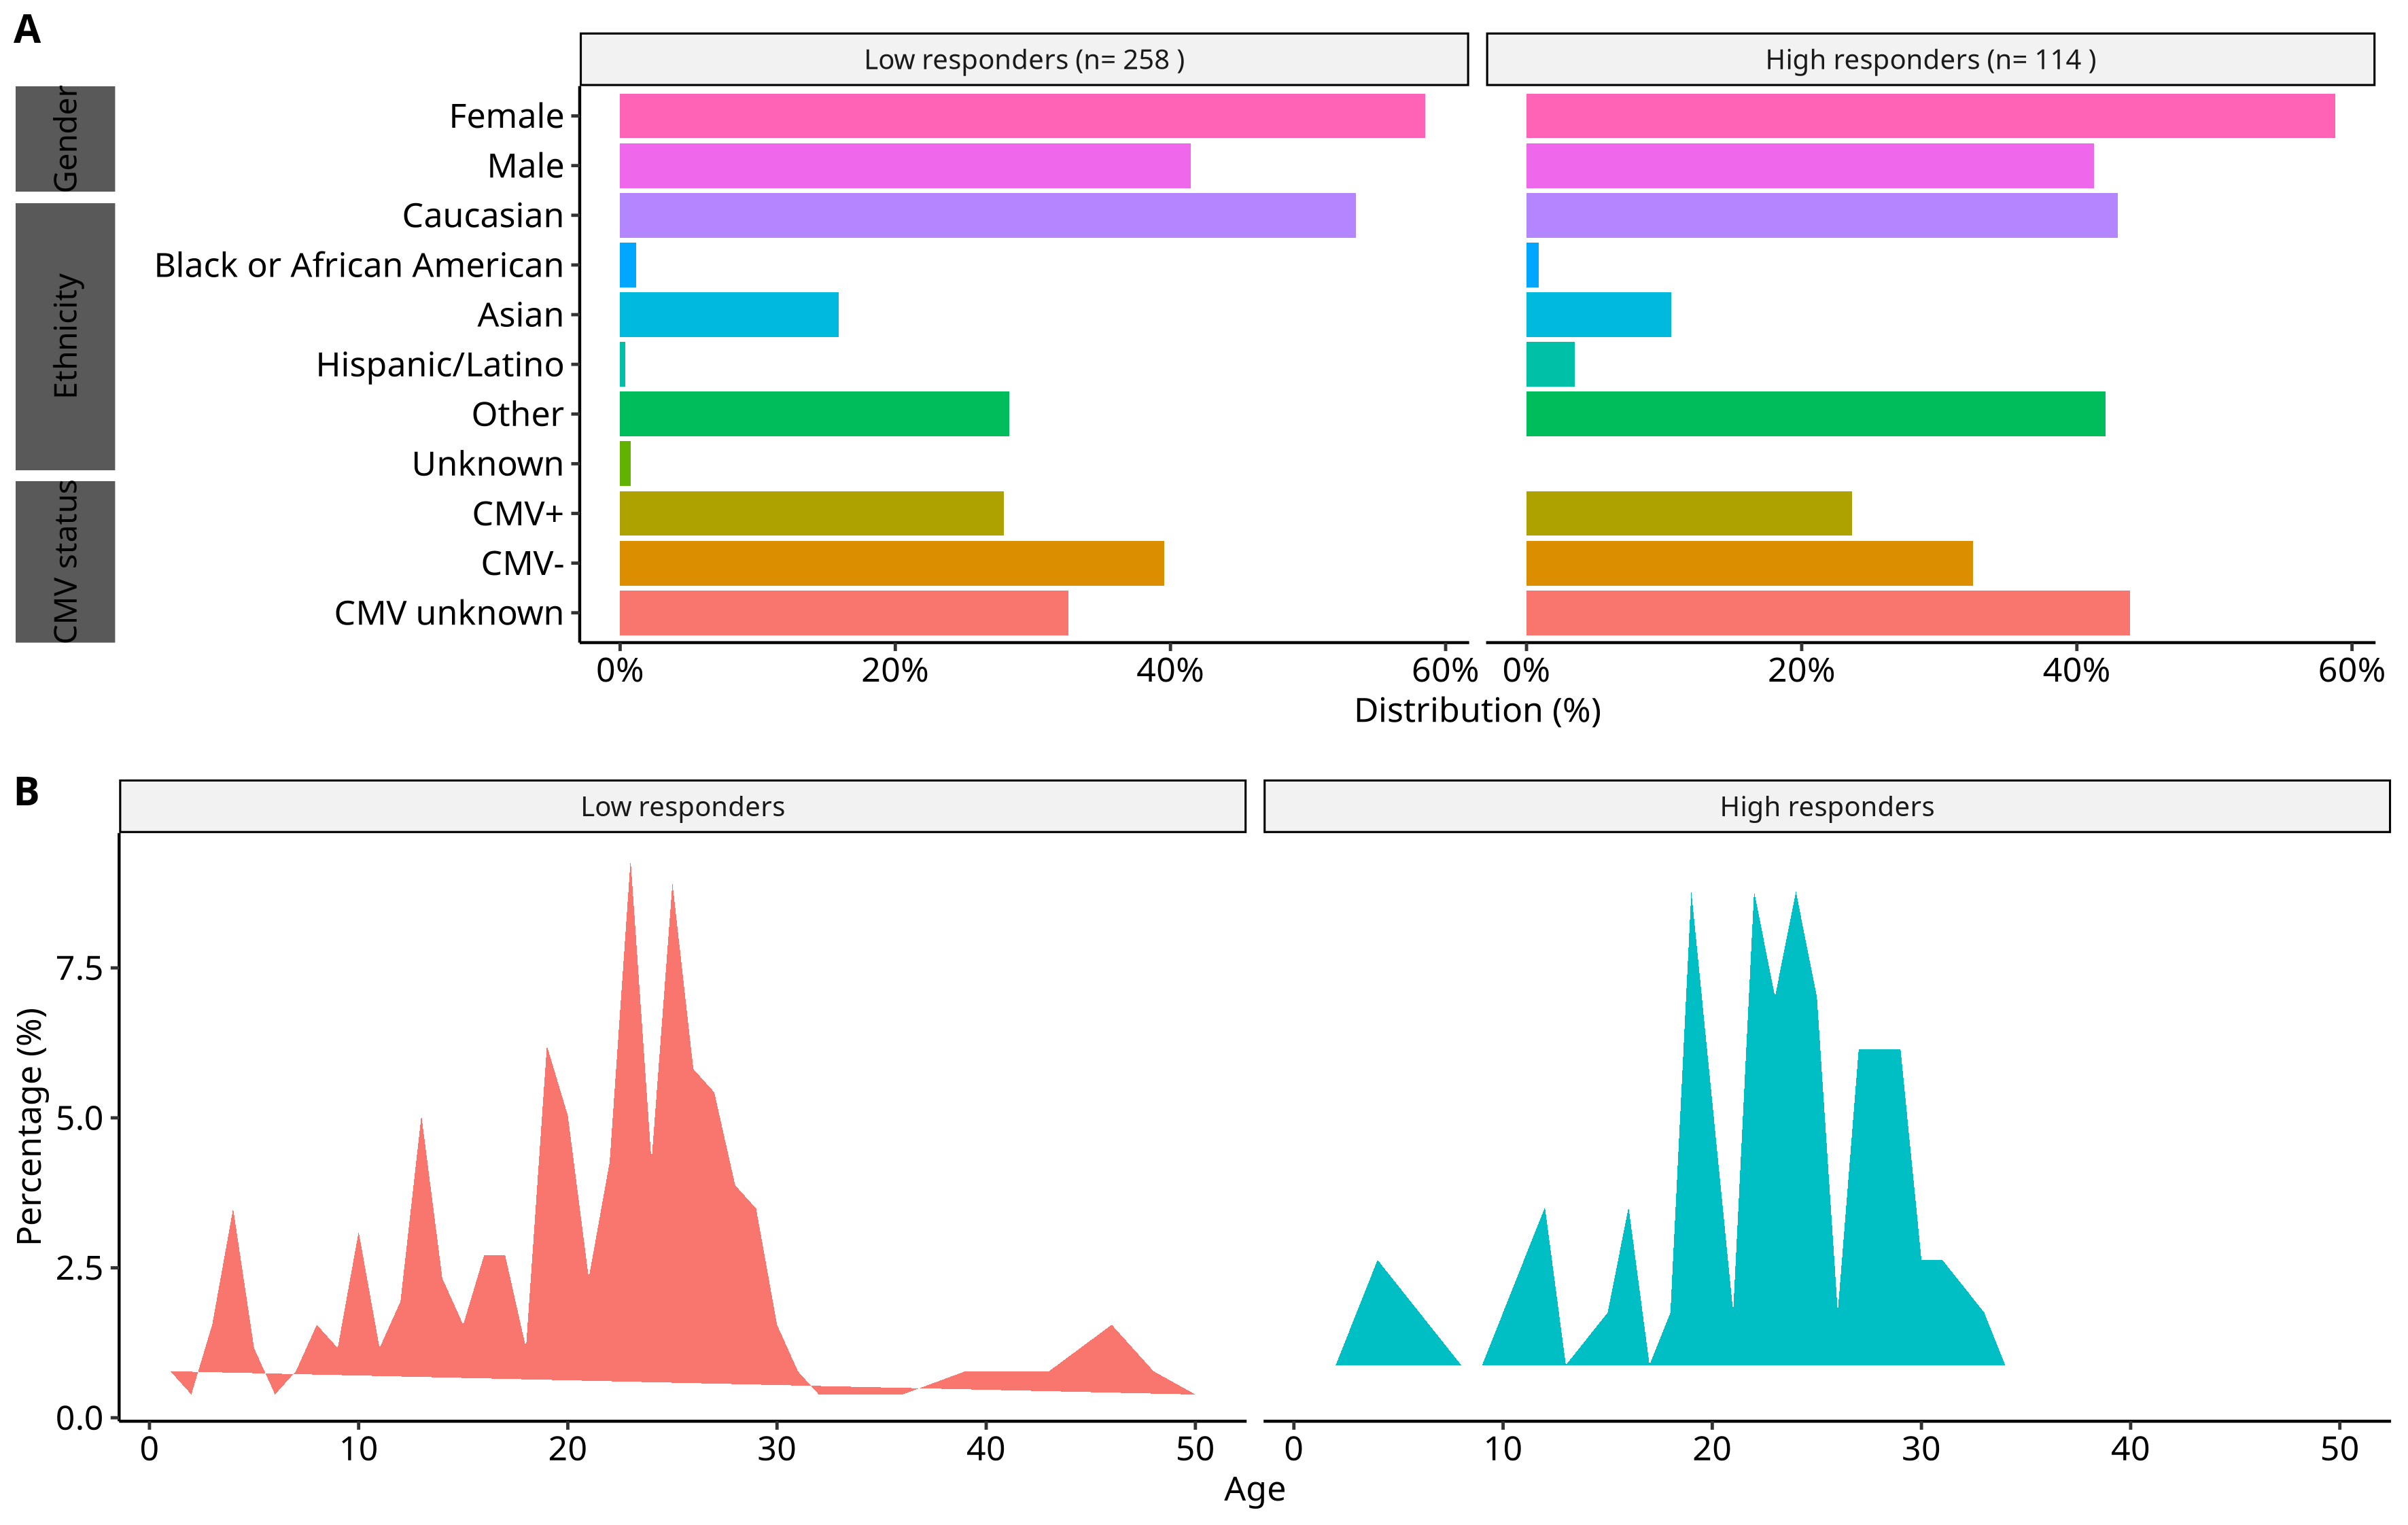
\includegraphics[width=\textwidth]{demographic}
    \caption{\textbf{A.} percentage of donors with factor property within high
    and low responder groups. Included are sex, race, and CMV status
    information. \textbf{B.} Age distribution of donors with a known response
    classification.}\label{fig:demoGraph}
\end{figure}



\begin{table}
\centering
\begin{tabular}{ll}
\toprule
\textbf{Age (y)} & \\
\midrule
Mean $\pm$ SD & 21.02 $\pm$ 8.66\\
Median (min. to max. range) & 22.5  ( 1 - 50 )\\
\addlinespace
    \textbf{Gender} & \\
\midrule
Male (\%) & 154 ( 41.4 )\\
Female & 218  ( 58.6 )\\
\addlinespace
    \textbf{Ethnicity} & \\
\midrule
Caucasian (\%) & 187 ( 50.3 )\\
African American (Black) (\%) & 4  ( 1.1 )\\
Asian (\%) & 53  ( 14.2 )\\
Hispanic/Latino (\%) & 5  ( 1.3 )\\
Other (\%) & 121  ( 32.5 )\\
Unknown (\%) & 2  ( 0.5 )\\
\bottomrule{}
\end{tabular}
\caption{\textbf{Demographic statistics of donors with known vaccine response classification.}}\label{tbl:demoStats}
\end{table}

\fptable{studies_table}{.7}
{Reference table of clinical studies}
{Clinical study ID used (but remapped) in the database, age information,
vaccine type information, and assay data types of clinical studies are in the
rest of the columns.}
{tbl:studiesDesc}


The data from the clinical studies consisted of 121 CSV files that were
imported into the FluPrint database. The data was used to build four tables
which will be described in the next sections, but we will not discuss technical
validation of the database construction, refer to the original work for that
\citep{tomicFluPRINTDatasetMultidimensional2019}.  The relation between the
tables is best visualised in the original work of
\citep{tomicFluPRINTDatasetMultidimensional2019}, it describes the MySql
attribute types and columns in the tables \autoref{fig:tablesFluprint}
(copied). The volume of the data is also given in the original work, per table
the number of rows and columns is reported \autoref{tbl:volumeTables}.

\begin{figure}
    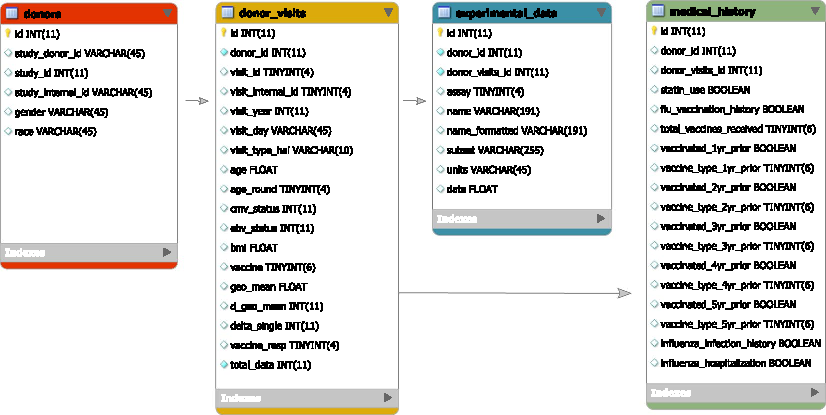
\includegraphics[width=\textwidth]{tablesFluprint}
    \caption{
        \textbf{(taken from original paper)} The FluPRINT database model. The diagram shows a schema of the FluPRINT
    database. Core tables, donors (red), donor\_visits (yellow),
    experimental\_data (blue) and medical\_history (green) are interconnected.
    Tables experimental\_data and medical\_history are connected to the core
    table donor\_visits. The data fields for each table are listed, including
    the name and the type of the data. CHAR and VARCHAR, string data as
    characters; INT, numeric data as integers; FLOAT, approximate numeric data
    values; DECIMAL, exact numeric data values; DATETIME, temporal data values;
    TINYINT, numeric data as integers (range 0–255); BOOLEAN, numeric data with
    Boolean values (zero/one). Maximal number of characters allowed in the data
    fields is denoted as number in parenthesis.
    }\label{fig:tablesFluprint}
\end{figure}

\begin{table}
    \centering
    \begin{tabular}{lll}
        \toprule{}
        \textbf{Table name} & \textbf{Rows} & \textbf{Columns} \\
        \midrule{}
        \textit{donors} &  740 & 6 \\
        \textit{donor\_visits} & 2,937 & 18 \\
        \textit{experimental\_data} & 371,260 & 9 \\
        \textit{Medical history} & 740 & 18 \\
    \bottomrule{}
    \end{tabular}
    \caption{Volume of tables in the Fluprint database.}\label{tbl:volumeTables}
\end{table}

\subsection{Attribute types and values}

Because of the great number of attributes in the database, we discuss them by
table starting with the donors \autoref{fig:tablesFluprint}.

\subsubsection{donors table}

The \textit{donors.id} attribute is simply an enumeration of unique donors,
importantly, it is used as a key to get attributes from other tables. The
column \textit{study\_donor\_id} is an encrypted identification number. Each
donor belongs to the study identified by the \textit{study\_id}, these are the
last two digist of the name code (those starting with SLVP0 \(\cdot\cdot\)) in
the reference table \autoref{tbl:studiesDesc}, the \textit{study\_internal\_id}
is either the digit or a string containing the digit in \textit{study\_id}. The
\textit{gender} and \textit{race} attribute contain the values used in
\autoref{fig:demoGraph}, a minor note is that in the original paper "American
Indian or Alaska Native" is listed as one of the \textit{race} values but is
not used in the database. There are 5 donors whose race is "NULL", which are
mapped to unkown \autoref{fig:demoGraph}.

\begin{table}
    \begin{tabular}{rlrlll}
\toprule{}
id & study\_donor\_id & study\_id & study\_internal\_id & gender & race\\
\midrule{}
1 & e27ad74ff9a5f2f32d8e852533f054c0 & 30 & 30 & Female & Asian\\
2 & 4a89ac4d3f4dc869e5c8e8cf862cffda & 30 & 30 & Male & Other\\
3 & a2cde6e54dec92422b0427dd49244350 & 30 & 30 & Female & Caucasian\\
4 & 0f7d8d1c13e876017ea465f99d25581f & 30 & 30 & Male & Other\\
5 & 1ed2f6409584b7b4e9720b28d794fe91 & 30 & 30 & Female & Caucasian\\
\addlinespace
6 & a575678405e9615bfb87eccfa031f7fc & 30 & 30 & Male & Other\\
\bottomrule{}
\end{tabular}
    \caption{Head of the donors table.}\label{tbl:donorsHead}
\end{table}

\subsubsection{donor\_visits table}

The donor visits table is the core table of the database, it contains donor
attributes at visit times during enrolment in clinical studies in rows that are
uniquely identified by an \textit{id} integer. Each
row also includes the \textit{donor\_id} identify the donor that visitted.

The database combines different clinical studies accross years and the data
from these studies is incomplete leading to an incomplete and hetergenous
database \autoref{tbl:visitsDesc}. For example some donors might miss their
second visit to determine their antibody levels, or the number of parameters
measured by an assay changed in the timespan of a clinical study. Unifying
these clinical studies in one database resulted in normalised but incomplete
data and heterogenous data. More specifically, every attribute in the core
table has missing value, which complicates dataset selection. One examples of
visit data of a donor is discussed to highlight important attributes and
problems in the data: that the number of visits is variable, that all columns
are incomplete, and that classification is sometimes based on single visits or
inconsistent \autoref{tbl:visit166} \autoref{tbl:visitsDesc}.

\begin{table}
\addtolength{\leftskip} {-2cm} % increase (absolute) value if needed
\addtolength{\rightskip} {-2cm} % increase (absolute) value if needed
\begin{tabular}{lrrrrrrrrr}
\toprule{}
stat & age & cmv\_status & ebv\_status & bmi & vaccine & geo\_mean & d\_geo\_mean & vaccine\_resp & total\_data\\
\midrule{}
n & 2937.0 & 1081.0 & 548.0 & 516.0 & 2794.0 & 984.0 & 1260.0 & 1206.0 & 2937.0\\
na & 0.0 & 1856.0 & 2389.0 & 2421.0 & 143.0 & 1953.0 & 1677.0 & 1731.0 & 0.0\\
mean & 47.3 & 0.4 & 0.8 & 24.8 & 3.7 & 87.6 & 8.9 & 0.3 & 126.4\\
sd & 27.0 & 0.5 & 0.4 & 5.6 & 1.0 & 101.7 & 30.9 & 0.4 & 368.4\\
se\_mean & 0.5 & 0.0 & 0.0 & 0.2 & 0.0 & 3.2 & 0.9 & 0.0 & 6.8\\
\addlinespace
IQR & 50.2 & 1.0 & 0.0 & 6.7 & 0.0 & 105.4 & 4.0 & 1.0 & 19.0\\
skewness & 0.2 & 0.3 & -1.4 & 1.0 & -1.7 & 3.6 & 9.9 & 1.1 & 7.1\\
kurtosis & -1.5 & -1.9 & -0.1 & 2.1 & 3.0 & 26.6 & 114.9 & -0.9 & 49.7\\
\bottomrule{}
\end{tabular}
\caption{Descriptive stats of relevant numeric or binary factor columns in the
    donor visits table. For geo\_mean 0 is considered as missing data.}\label{tbl:visitsDesc}
\end{table}

Per donor all visits are enumerated in chronological order by
\textit{visit\_id} \autoref{tbl:visit166}. Further visit info includes:
\textit{visit\_internal\_id} which is a number that indicates the visit order
within an influenza season but this differs per clinical study (e.g. some use
1-2-3, orther use 0-7-28), the \textit{vist\_year} is the influenza season of
the visit, the \textit{visit\_day} is the number of days relative to the date
of vaccination,  \textit{age} and \textit{age\_round} indicate the donor's age
at time of the visit, and \textit{bmi} gives the donor bmi at visit time, and
lastly \textit{visit\_type\_hai} is the intent of the visit which is either
"pre", "post", or "other",

During the "pre" visit a virological assay is performed to determine the CMV
and Epstein-Barr virus (EBV) status of the donor, which are indicated by the
binary variables \textit{cmv\_status} and \textit{ebv\_status}.

To measure vaccine response to a vaccine which is indicated by an id
\autoref{tbl:remapVaccine} in \textit{vaccine}, the hemagglutination inhibition
assay (HAI assay) is used. The procedure measures the influenza antibody titers
before vaccination during the \textit{visit\_type\_hai} "pre" visit of a
participant, and 28 days after vaccination during a "post" visit. The geometric
mean titer (GMT) at each visit is calculated, and a fold change in GMT is
calculated as the ratio of the GMT at day 28 (post) and during the first visit
(pre). These values are \textit{geo\_mean} and \textit{d\_geo\_mean},
\textit{d\_single} is the antibody titer fold-change per strain of virus used
in the vaccine, it is unclear how this value is aggregated over different
strains and is left out of further analysis.  This data was used to classify
donors in high or low responders according to FDA guidelines \cite{},
individuals are high-responders if they seroconverted (4-fold or greater rise
in HAI titer) and were seroprotected (GMT HAI \(\ge\) 40) after vaccination.
The seasonal vaccine response classifications are given by the binary variable
\textit{vaccine\_resp}.

The assays performed to get a serological/immunlogical profile of the donor
before vaccination are described later in the section of the experimental data
table, all assays are listed in the original work
\cite{tomicFluPRINTDatasetMultidimensional2019} and are summarised here
\autoref{tbl:assays}, the total rows of assay data is given by
\textit{total\_data}.

\begin{table}
\addtolength{\leftskip} {-2cm} % increase (absolute) value if needed
\addtolength{\rightskip} {-2cm} % increase (absolute) value if needed
\begin{tabular}{rrrlrrrlrrrrr}
\toprule{}
visit\_id & year & day & type & age & cmv & ebv & bmi & vaccine & geo\_mean & d\_geo\_mean & response & assay\_data\_rows\\
\midrule{}
1 & 2011 & 0 & pre & 20 & 1 & 1 & 30.31 & 4 & 25.20 & 6 & 0 & 343\\
2 & 2011 & 7 & other & 20 & 1 & 1 & NULL & 4 & 0.00 & 6 & 0 & 51\\
3 & 2011 & 28 & post & 20 & 1 & 1 & NULL & 4 & 160.00 & 6 & 0 & 51\\
4 & 2012 & 0 & pre & 21 & 1 & 1 & 30.31 & 4 & 9.28 & 4 & 0 & 292\\
6 & 2013 & 0 & pre & 22 & 1 & 1 & 30.31 & 4 & 15.91 & 2 & 0 & 2877\\
\addlinespace
7 & 2013 & 7 & other & 22 & 1 & 1 & NULL & 4 & 0.00 & 2 & 0 & 63\\
8 & 2013 & 28 & post & 22 & 1 & 1 & NULL & 4 & 26.75 & 2 & 0 & 82\\
\bottomrule{}
\end{tabular}
\caption{Visit data of donor 166 from study SLVP021 \autoref{tbl:studiesDesc},
where participants are only vaccinated once.
Number of visits and data collected at visit varies, classification is
inconsistent with \( \geq 40\) and 4-fold increase
rule in 2011.}\label{tbl:visit166}
\end{table}

The most important data related to the visits of donor 166 is shown in Table
\ref{tbl:visit166}.  The vaccine response classification is calculated based on
the GMT in the "pre" and "post" visits.  This classification is done per
influenza season, but the HAI assay requires a "pre" visit and a "post" visit
28 days later to measure the difference in GMT.  However, sometimes a
classification is given when there is only one visit record in a season, like
in 2012 for donor 166 \autoref{tbl:visit166}.

\begin{figure}
    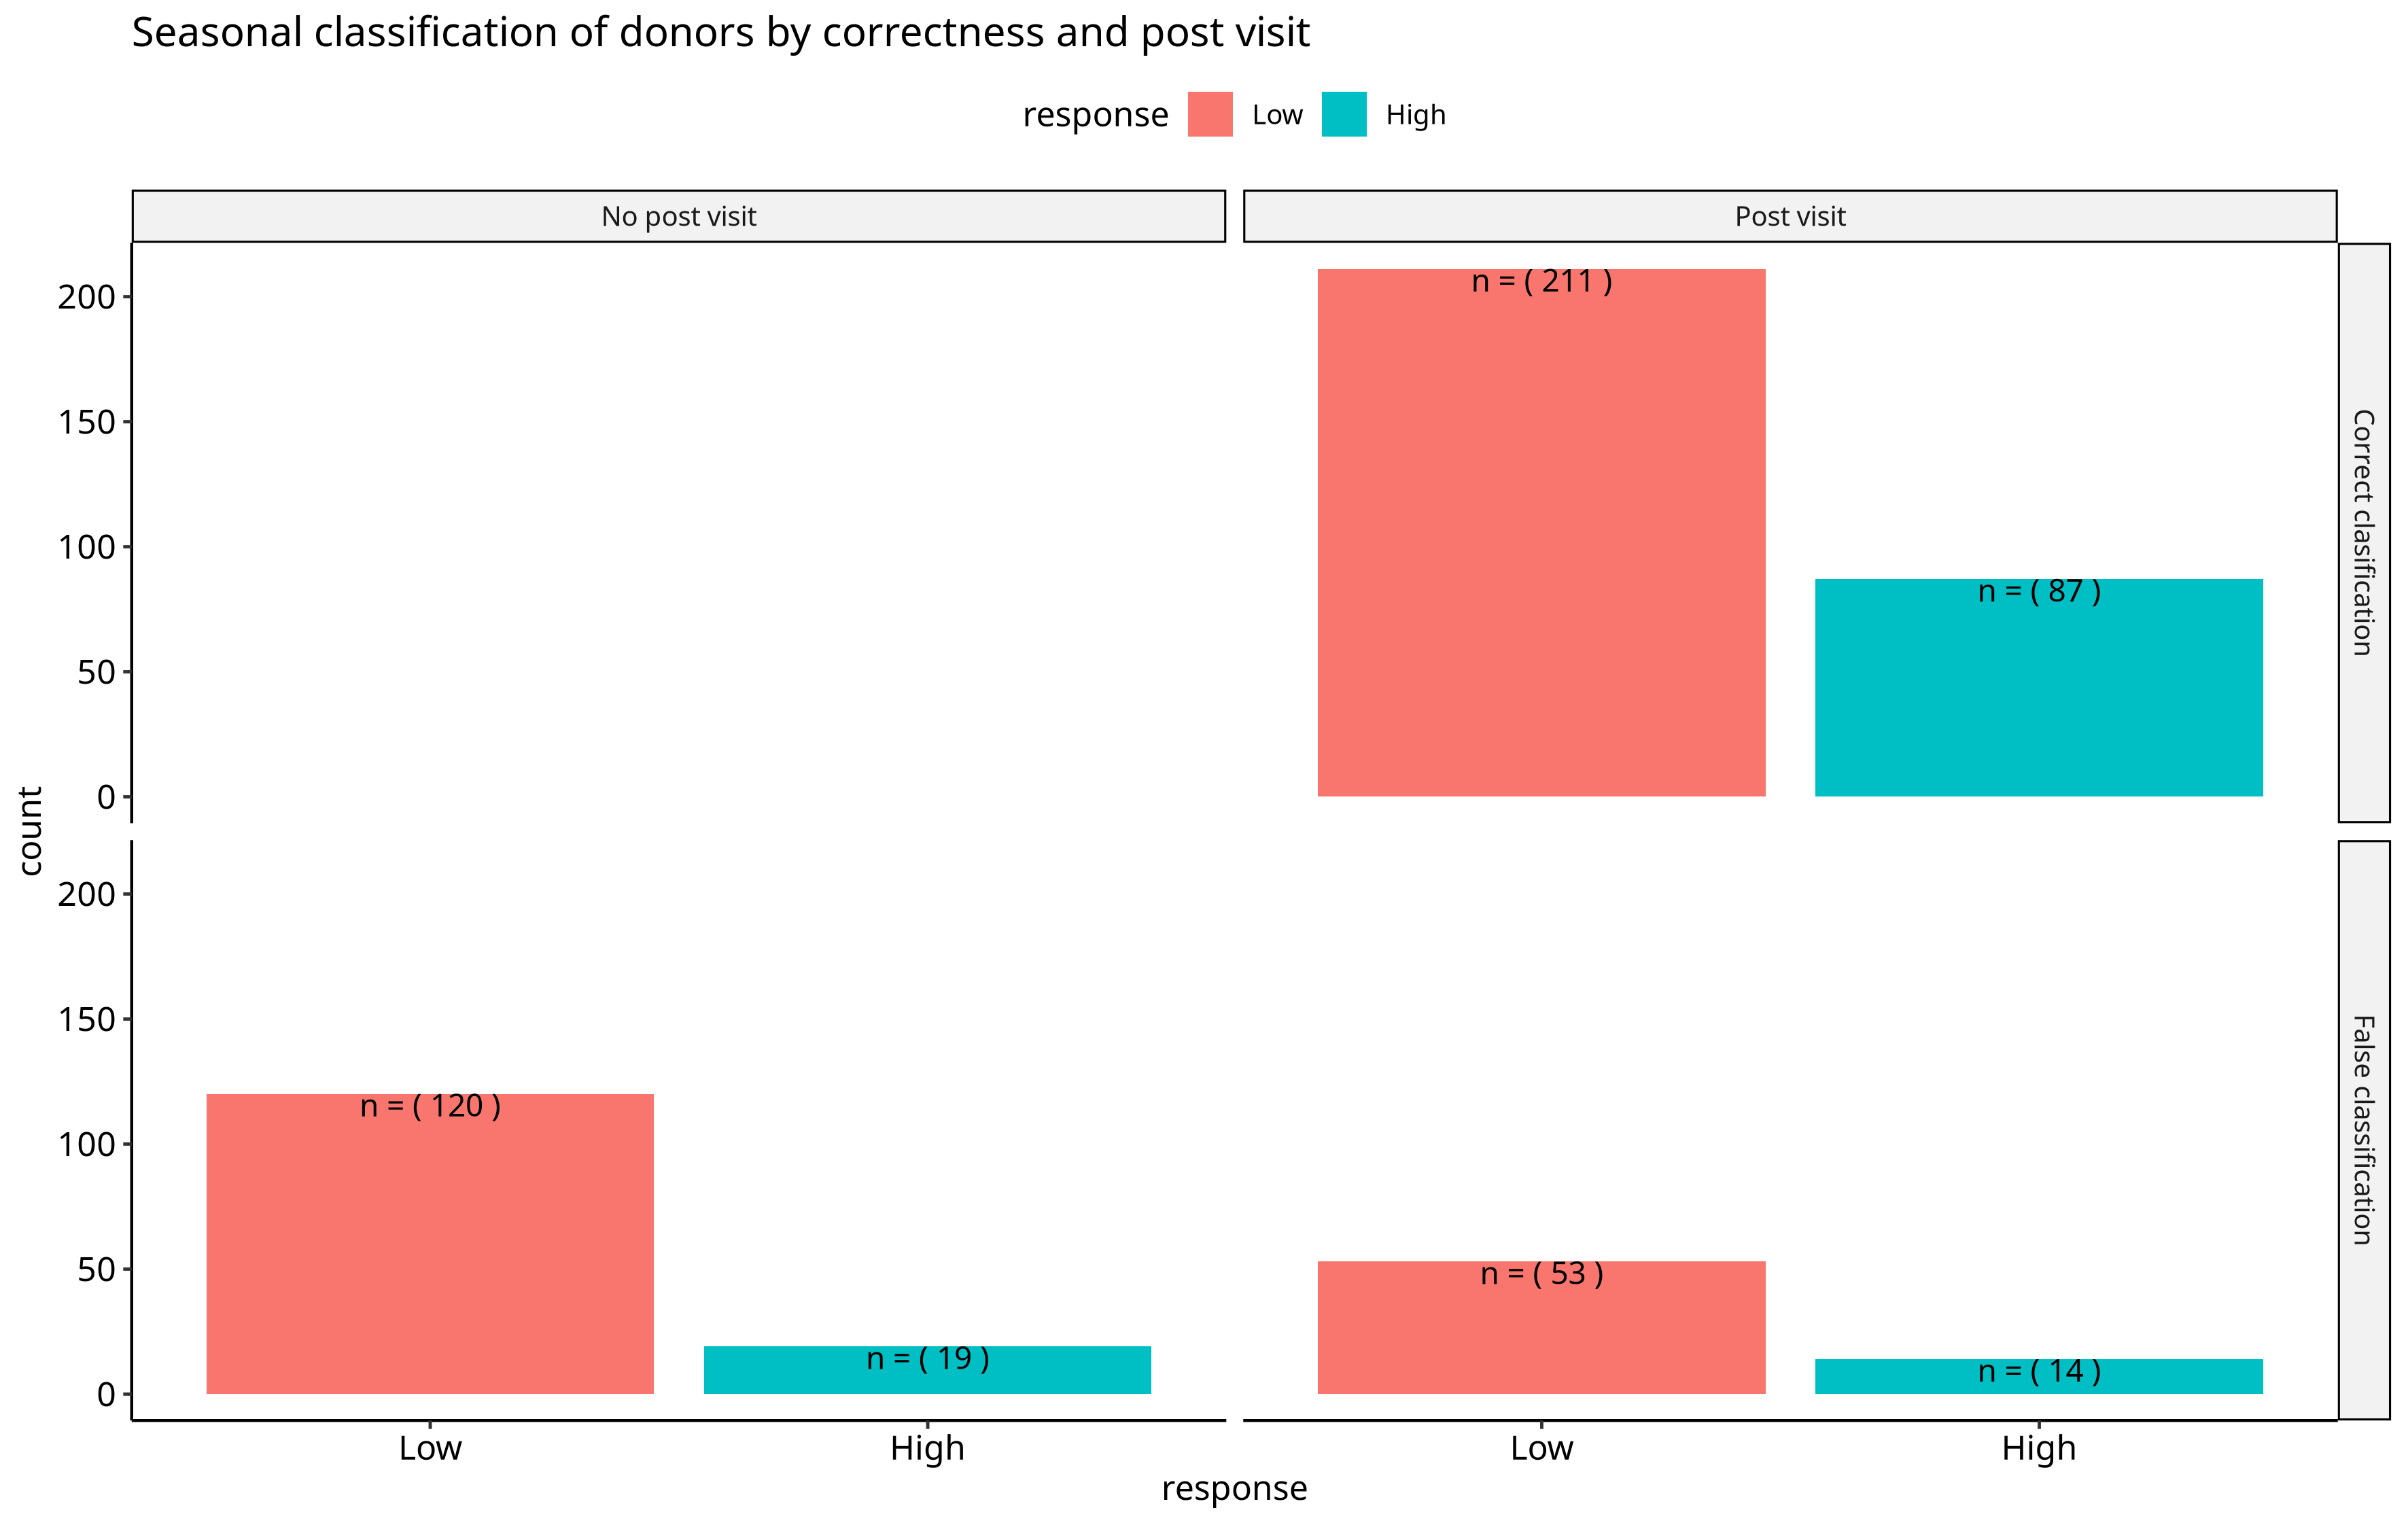
\includegraphics[width=\textwidth]{season_classification}
    \caption{}\label{fig:classInconsistent}
\end{figure}

The example of donor 166 contains an inconsistency in the classification, in
2011 the GMT \textit{geo\_mean} increases from 25.20 to 160.00, and the
\textit{d\_geo\_mean} is 6, but in this season the donor is wrongly classified
as a low responder \autoref{tbl:visit166}. Because of this the seasonal
classification of donors was investigated using the seroprotection and
seroconversion criteria \ref{fig:seasonalClasses}, records of incorrectly
labelled donors are also saved as a spreadsheet.

\subsubsection{Experimental data table}

\begin{table}
    \begin{tabularx}{\textwidth}{Xp{0.5\textwidth}X}
\toprule{}
        \textbf{Name} & \textbf{Description} & \textbf{id} (\textit{experimental\_data.assay})\\
\midrule{}
        (Multiplex) cytokine assays & Multiplex ELISA using Luminex polysterene
        bead or magnetic bead kits. Measures serum cytokine/hormone level in
        z.log2 units using fluorescent antibodies. & 3, 6, 15, 16\\
        \addlinespace
        Flow and mass cytometry assays & uses labeled antibodies to detect antigens on
        a cell surface to identify a subset of a cell population, units are in
        percentage of parent population. & 4, 9, 13, 17 \\
        \addlinespace
        Phosphorylation cytometry assays & Uses antibodies to measure
        phosphorylation of specific proteins stimulated by an immune system event
        belonging to cell population subsets. Units are a fold change between
        stimulated and un-stimulated cells, for mass cytometry arcsin readout difference,
        fold-change of 90th percentile readout values otherwise.  & 7, 10 (mass cytometry) (flow cytometry)\\
        \addlinespace
        complete blood count (CBCD) & Different cells are counted using flow
        cytometry Units are usually in Count/$\mu$L & 11 \\
        \addlinespace
        meso scale discovery assays (MSD) & A setup where serum cytokines or hormones
        are captured with antibodies, and then detected by using a detection
        antibody. Units are arbitrary intensity & 2, 12, 14 \\
\bottomrule{}
\end{tabularx}
    \caption{assays table}\label{tbl:assays}
\end{table}


Assays performed in visits are remapped, but the values in the
database do not correspond to the reported table \autoref{tbl:remapVaccine}.
Actual assay type, data units, and id in the database are reported here
\autoref{tbl:assays}.

\fpfig{exp_data_numbers}{.7}
{Feature count per individual assay id, assay type, stratisfied in either response status or study}
{caption}
{fig:featureNumbers}

In total there are data from 14 different assays, not counting the virological
and HAI antibody assays \autoref{tbl:assays}. The virological assays include
the cmv virus status and ebv status, and is not used in this work because it is
done in a smaller subset of studies. Those 14 assays have been aggregated in
this work to 5 different types of experiments: the multiplex assays measure
serum molecules such as cytokines and other signaling molecules, flow and mass
cell cytometry measure the phenotype of specific immune related cells,
phosphorylation flow and mass cytometry measures the phosphorylation signaling
pathway activation after an immune stimulation, the blood count measures the
count of cells in the blood, and meso scale discovery (MSD) measures hormones
or cytokines from the blood.

\begin{figure}
    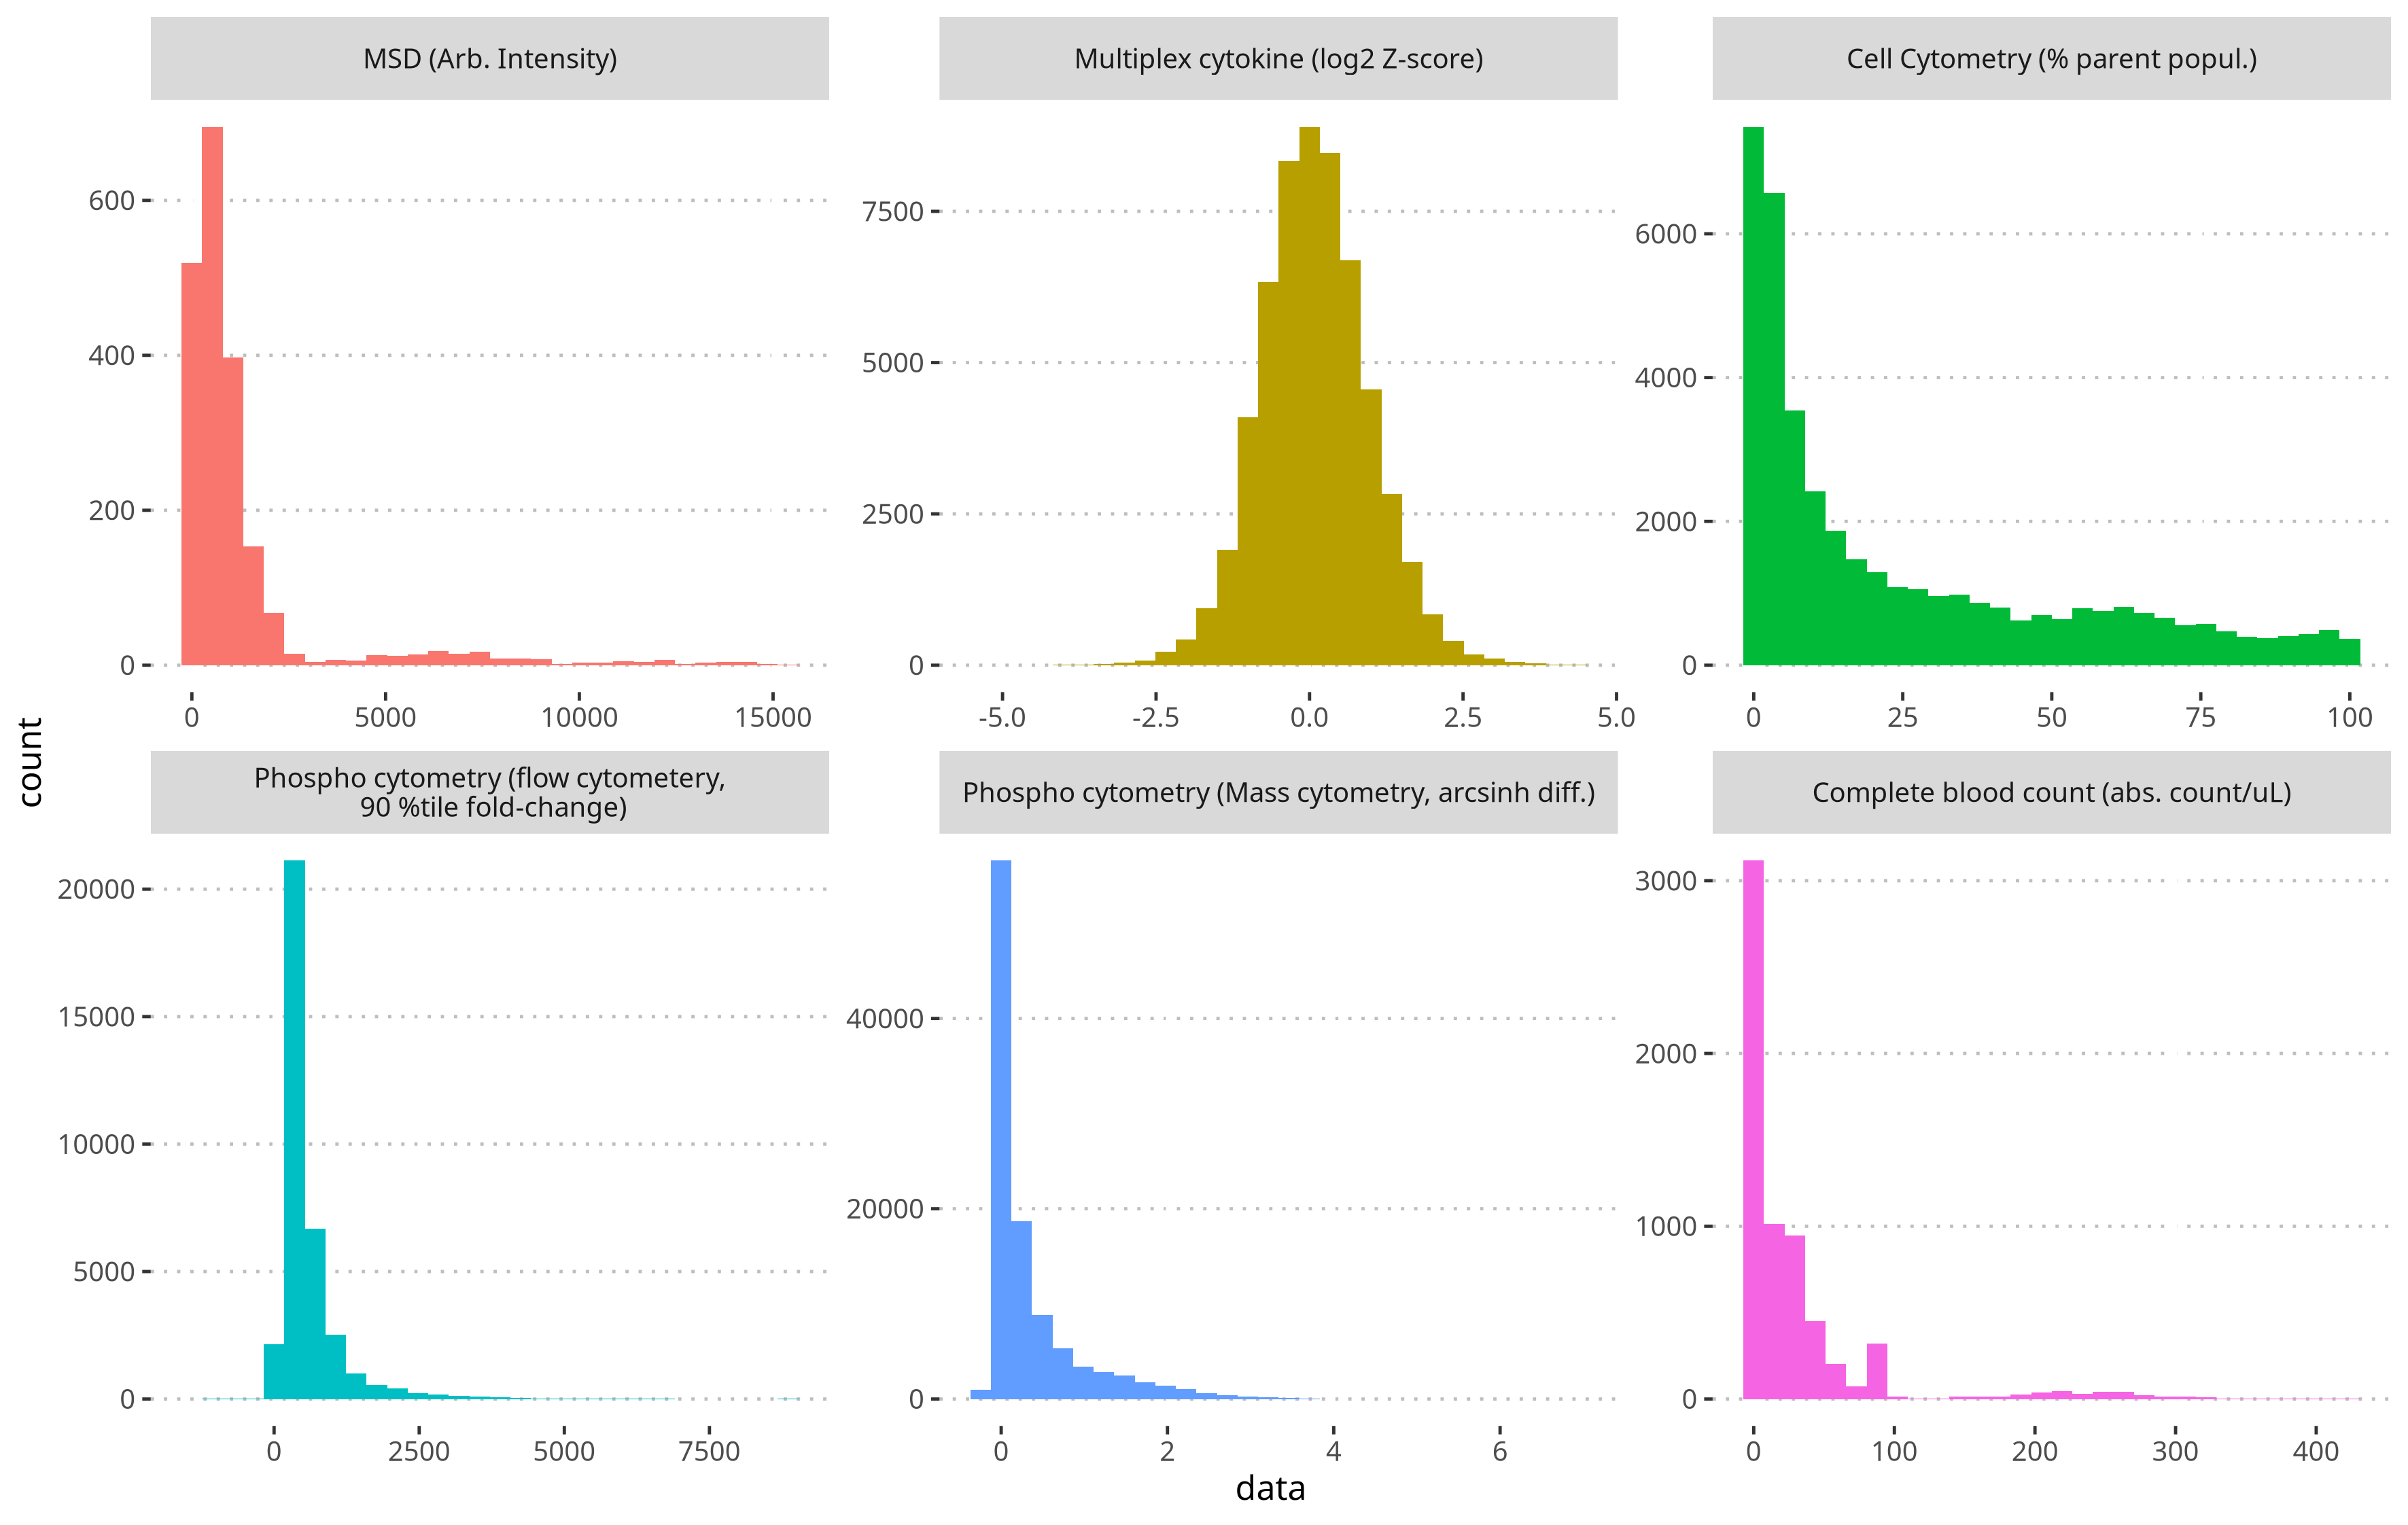
\includegraphics[width=\textwidth]{assay_value_distributions}
    \caption{noise in 90th \%tile}\label{fig:assayDistr}
\end{figure}

The experimental data table contains all features recorded for a donor visit.
The number of features collected for each visit is large and varies greatly
(mean at 126 , \(\pm \)368 SD) \autoref{tbl:visitsDesc}, and in total there are
3285 different features measured across all clinical studies. However, not
every assay is done in every clinical study \autoref{fig:featureNumbers} and
over the years the data generated by assays has changed, so a table with all
features as columns and all donors as rows would be extremely sparse (and
crashes R due to RAM limitations).  Describing the 3285 different
features in this sparse table would be impossible, but assay value
distributions across studies are shown to follow normal or power distributions
\autoref{fig:assayDistr}. Global correlation analysis is complicated by the
great number of features and sparseness in the data.

\begin{figure}
    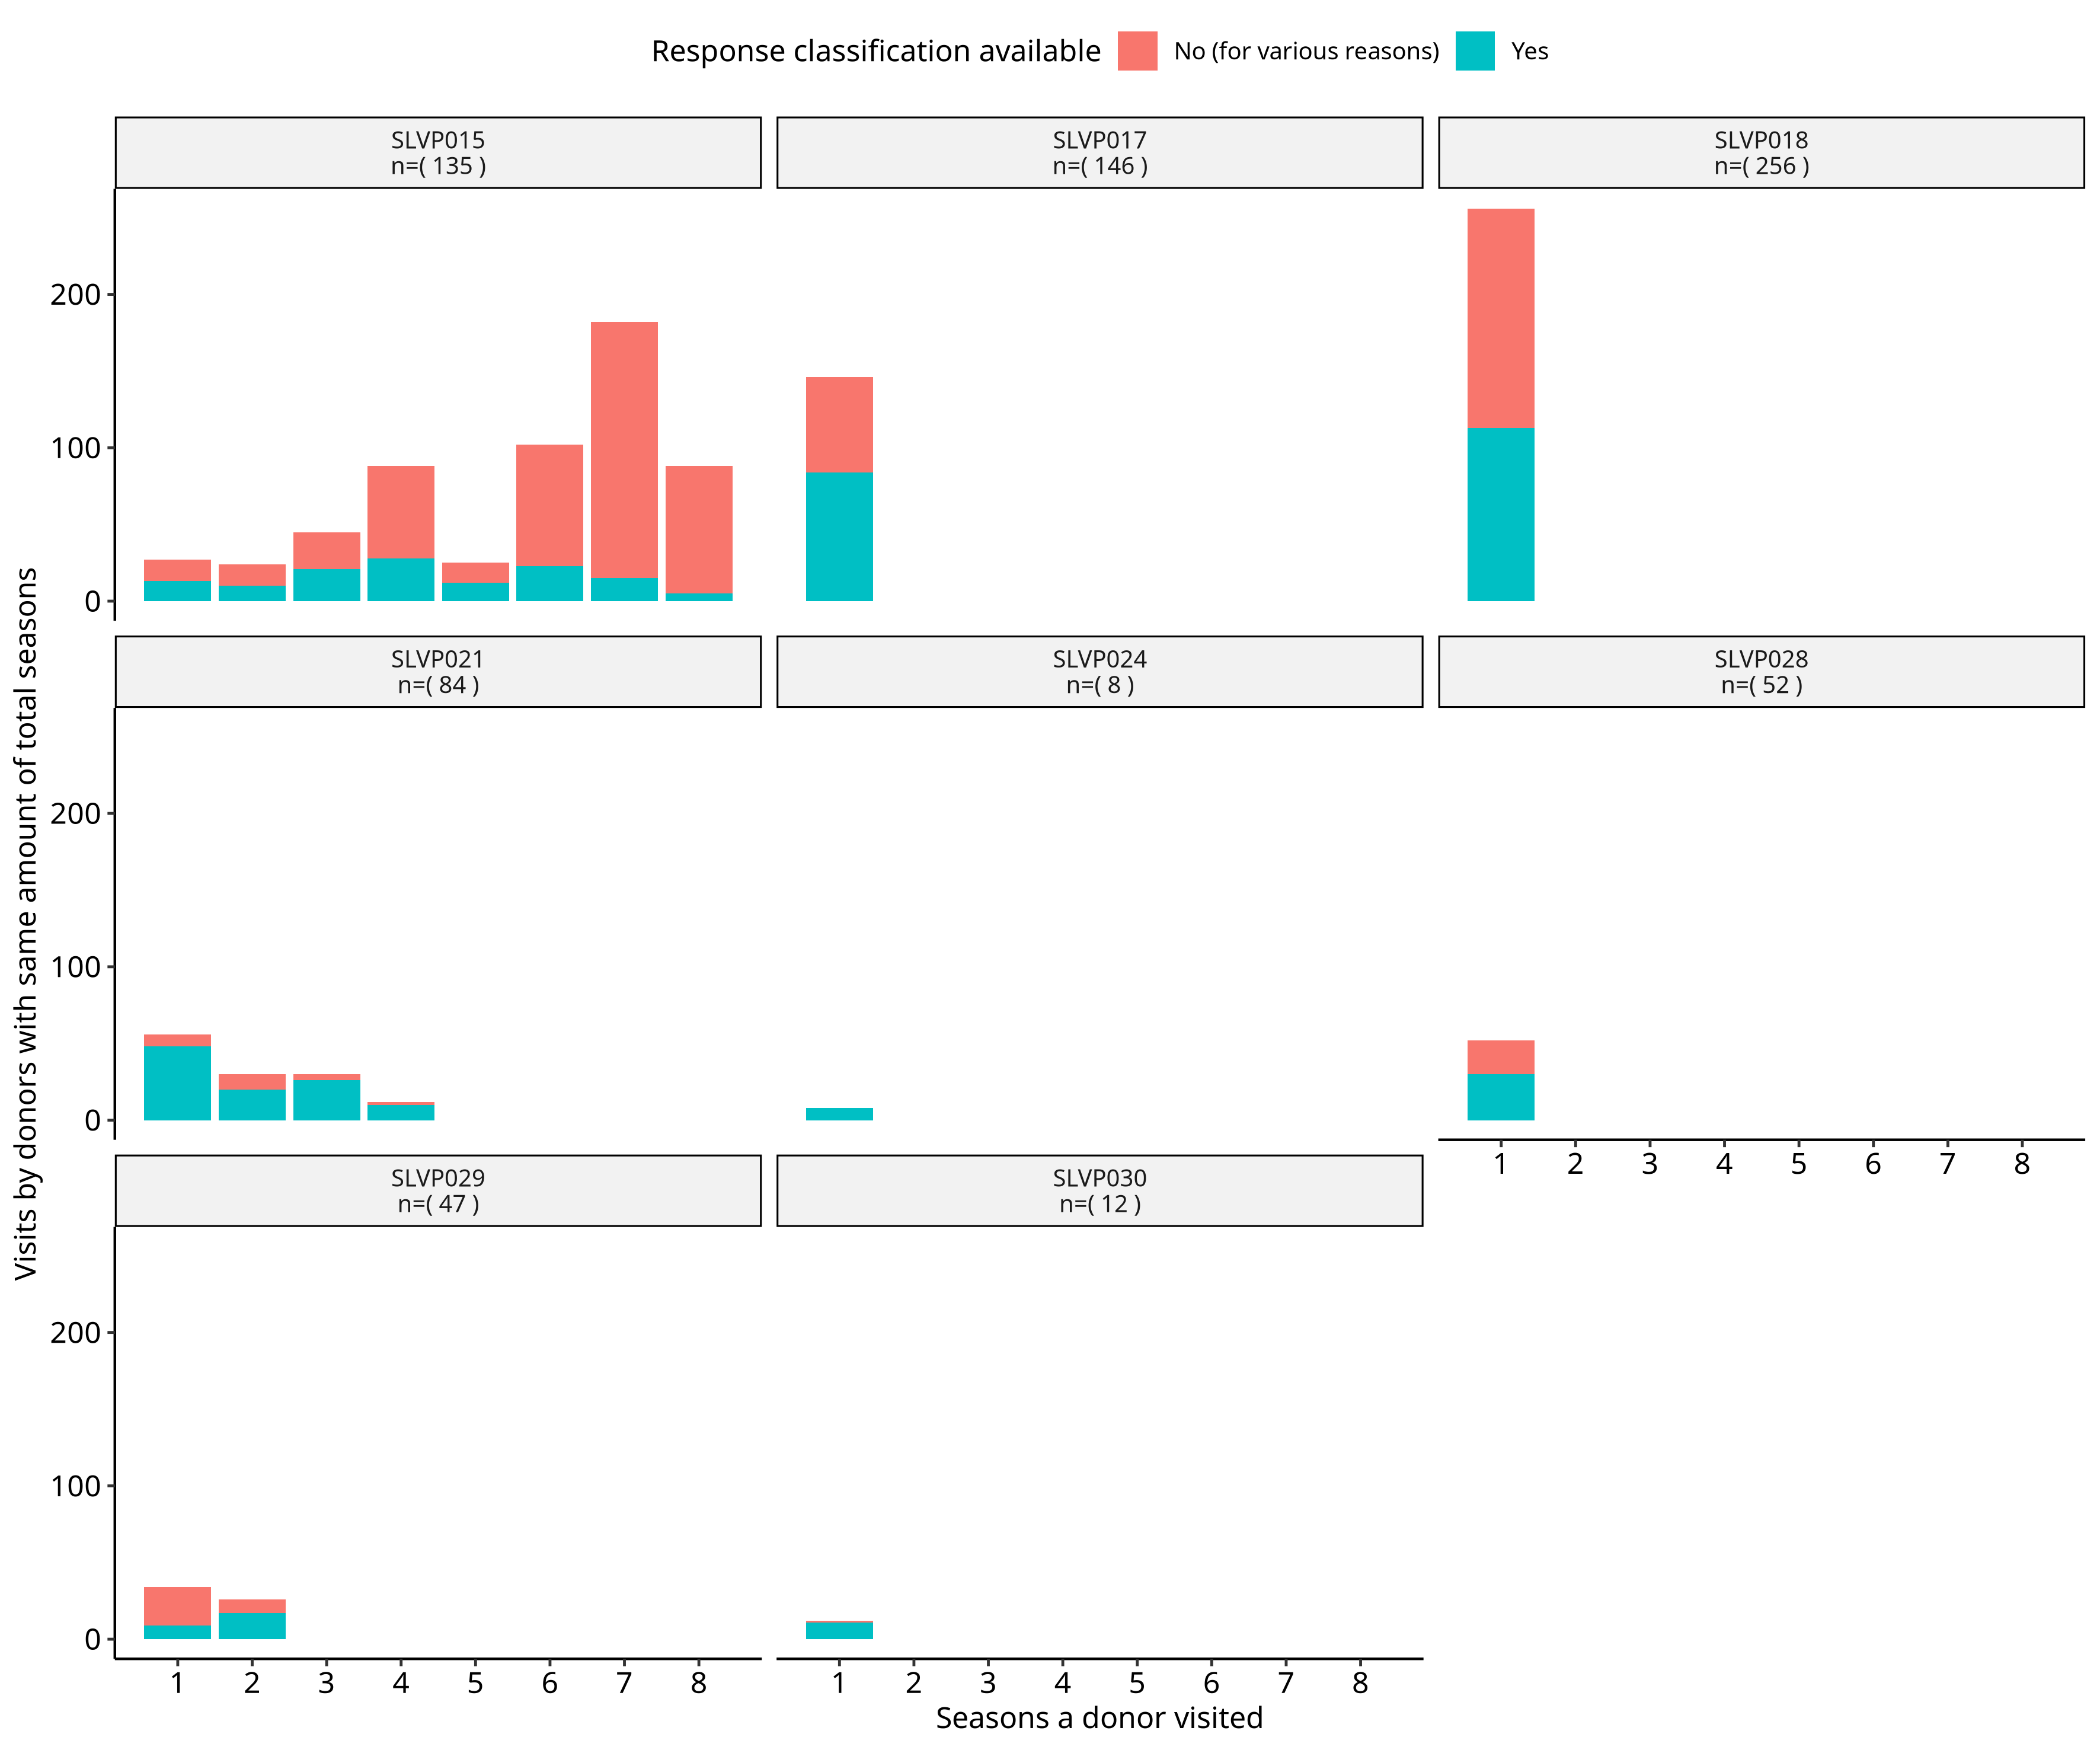
\includegraphics[width=\textwidth]{repeat_visits_per_study}
    \caption{the number of donors that visited per number of influenza seasons
    they visited (years), per study. The color indicates the number of visits for which a
    classification was available, counted within the groups of donors that
    visited the same amount of times.}\label{fig:repeatVisits}
\end{figure}

What further complicates selecting data is repeat visits of donors, and missing
visits. The problem of repeat visits over a span of multiple influenza seasons
is that not the same assay types are done, and that repeat visits are only a
small portion of the database. The data is also not suitable right away for
studying the effect of repeat vaccination on high versus low vaccine reponse,
since the classification in the longitudal study (SLVP015) is mostly not
available \autoref{fig:repeatVisits}.

For example exploring the effect repeat vaccination has an response rate would
first require manual labelling of high and low responses, at least for the
cases where it is possible based on the GMT data. Those cases are when
classification is set to a null value even though GMT data is available.  The
reason for this null value assignment is reported, but the pattern seems to set
the vaccine response to null if there is not enough assay data measured.

\section{Data quality}

The database has issues that are inherent to combining multiple studies and the
classification is inconsistent in some cases \autoref{fig:classInconsistent},
or often missing completely because no HAI antibody assay data was available or
the classification was set to a null value by the database authors
\autoref{fig:repeatVisits}.  The main value of the database is the assay data
that is fully represented in all studies and across all years, but this
information is hard to access since all studies do not use overlapping assays
\autoref{fig:featureNumbers}, resulting in high sparsity data. Further, the
sample size that can be used for further studies is limitted, since the high
versus low vaccine response is only available for a small subset of the data.

Specific attributes that have great amounts of missing values are the
virological and HAI assay data, the last is used for the vaccine response
classifcation. Potential for Studying the correlation of these values with
vaccine response is thus limitted. Nevertheless assay data is often available
and could be used to identify immunological factors that correlate with other
data, such as repeat vaccination, the exploration of this effect is outside the
scope of this work due to the data sparsity issues.

\printbibliography

\begin{appendices}
    \section{Remaps used in the database}

    \begin{table}[h]
        \begin{tabular}{lll}
            \toprule{}
            Vaccine received & Vaccine type ID & Vaccine type name \\
            \midrule{}
            FluMist IIV4 0.2 mL intranasal spray & 1 & Flumist \\
            FluMist Intranasal spray & 1 & Flumist \\
            FluMist Intranasal Spray 2009–2010 & 1 & Flumist \\
            FluMist Intranasal Spray & 1 & Flumist \\
            Flumist & 1 & Flumist \\
            Fluzone Intradermal-IIV3 & 2 & Fluzone Intradermal \\
            Fluzone Intradermal & 2 & Fluzone Intradermal \\
            GSK Fluarix IIV3 single-dose syringe & 3 & Fluarix \\
            Fluzone 0.5 mL IIV4 SD syringe & 4 & Fluzone \\
            Fluzone 0.25 mL IIV4 SD syringe & 5 & Paediatric Fluzone \\
            Fluzone IIV3 multi-dose vial & 4 & Fluzone \\
            Fluzone single-dose syringe & 4 & Fluzone \\
            Fluzone multi-dose vial & 4 & Fluzone \\
            Fluzone single-dose syringe 2009–2010 & 4 & Fluzone \\
            Fluzone high-dose syringe & 6 & High Dose Fluzone \\
            Fluzone 0.5 mL single-dose syringe & 4 & Fluzone \\
            Fluzone 0.25 mL single-dose syringe & 5 & Paediatric Fluzone \\
            Fluzone IIV3 High-Dose SDS & 6 & High Dose Fluzone \\
            Fluzone IIV4 single-dose syringe & 4 & Fluzone \\
            Fluzone High-Dose syringe & 6 & High Dose Fluzone \\
            \bottomrule{}
        \end{tabular}
        \caption{Remaps of vaccine type relevant to to the clinical studies
        reference table \autoref{tbl:studiesDesc}, and the section on the donor
        visits table.}\label{tbl:remapVaccine}
    \end{table}

    \begin{table}
        \begin{tabular}{ll}
            \toprule{}
            Original & Remapped \\
            \midrule{}
            No& 0 \\
            Yes& 1 \\
            IIV injection/im& 2 \\
            Doesn’t know/doesn’t remember/na/does not remember& 3 \\
            LAIV4 intranasal/laiv\_std\_intranasal/laiv\_std\_ intranasal/nasal/intranasal& 4 \\
            \bottomrule{}
        \end{tabular}
        \caption{caption}\label{tbl:remapHistory}
    \end{table}

    \begin{table}
        \begin{tabular}{ll}
            \toprule{}
            Original & Remapped \\
            \midrule{}
            CMV EBV & 1 \\
            Other immunoassay & 2 \\
            Human Luminex 62–63 plex & 3 \\
            CyTOF phenotyping & 4 \\
            HAI & 5 \\
            Human Luminex 51 plex & 6 \\
            Phospho-flow cytokine stim (PBMC) & 7 \\
            pCyTOF (whole blood) pheno & 9 \\
            pCyTOF (whole blood) phospho & 10 \\
            CBCD & 11 \\
            Human MSD 4 plex & 12 \\
            Lyoplate 1 & 13 \\
            Human MSD 9 plex & 14 \\
            Human Luminex 50 plex & 15 \\
            Other Luminex & 16 \\
            \bottomrule{}
        \end{tabular}
        \caption{caption}\label{tbl:remapAssays}
    \end{table}
\end{appendices}

\end{document}
